\section{Tracking User Styles across Clear and Dark Web Forums}
\label{chp:stylometry_extensions:followingTrail}
The code to reproduce the following analysis is available on Github at the following URL:\\
 {\url{https://github.com/pranavmaneriker/ccc_darkweb_stylometry}}.

\subsection{Motivation}
\label{chp:stylometry_extensions:followingTrail:motivation}
In~\chapref{chp:sysml}, we described an architecture utilizing text CNNs~\citep{kim2014convolutional} for generating the textual component of representations for authorship attribution on darknet forums.
Recent work on generalizing authorship representations has focused on a variation of the popular sentence transformer architecture~\citep{reimers2019sentencebert}.
Specifically, \citet{riverastao2021learning} compared the transferability of author representation learning models between Amazon reviews, fanfiction short stores, and Reddit comments.
They found that in a zero-shot setting, i.e., without any addition in domain data, the models trained on Reddit data had the highest degree of generalization to new domains.
This work motivates us to explore the generalization capabilities of models trained on clear web data to dark web forums.
We explore two research questions.
First, can we apply author representation models trained on Reddit forum data directly to Darkweb forums?
Second, can we combine data from the dark web and clear web to build better models?

\subsection{Datasets}
\label{chp:stylometry_extensions:followingTrail:datasets}

\begin{figure}
    \centering
    \begin{subfigure}{0.9\linewidth}
       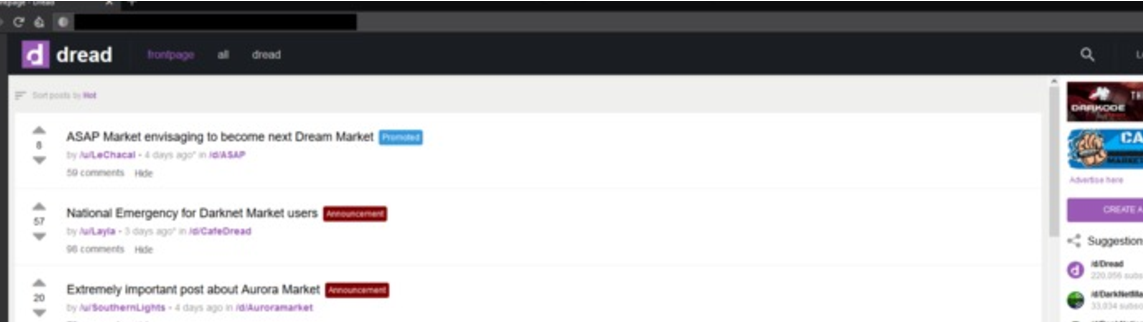
\includegraphics[width=\textwidth]{stylometryExtensions/figures/Dread} 
    \end{subfigure}
    \begin{subfigure}{0.9\linewidth}
       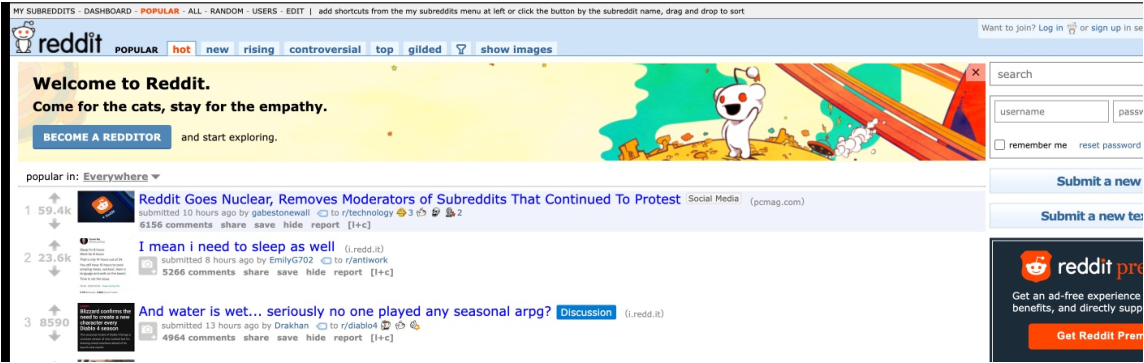
\includegraphics[width=\textwidth]{stylometryExtensions/figures/Reddit} 
    \end{subfigure}
    \caption{Dark web market Dread (top) and clear web market Reddit (bottom). Dread image source:~\citet{wiki:Dread}}
    \label{fig:stylometry_extensions:followingTrail:forums}
\end{figure}

\begin{table}
    \centering
    \begin{tabular}{cccc}
        \toprule
        Dataset &  \# Authors & \# Posts & \# Subforums\\
        \midrule
        Dread & 43,629 & 294,596 & 382 \\
        The Hub & 8,243 & 88,753 & 62 \\
        Reddit-201801 & 4,413,757 & 82,531,775 & 94,945 \\
        Reddit-201912 & 7,439,040 & 126,992,546 & 155,864 \\
        \bottomrule
    \end{tabular}
    \caption{Dataset statistics for comparing LUAR on clear and dark web forums.}
    \label{tab:stylometry_extensions:followingTrail:datasets}
\end{table}

To answer the research questions, we collect datasets from both clear and dark web forums.
For the clear web, we sample data from the Pushshift Reddit corpus~\citep{baumgartner2020pushshift}.
The LUAR model is trained on Reddit data sampled from the same corpus, but collected between 2015 and 2019.
To avoid any overlap with the training data, we sample data from 2018 and 2019.
We created two datasets, one for posts sampled from January 2018 and the second for posts sampled from December 2019.
Reddit is an `omni-forum'~\citep{munksgaard2016mixing}, where users can participate in a number of subcommunities (subreddit).
The similarity between Dread and Reddit is illustrated in Figure~\ref{fig:stylometry_extensions:followingTrail:forums}.
Keeping this in mind, we collect `omni-forums' from dark web data.
We collected datasets provided in the CrimeBB collection~\citep{pastrana2018crimebb} and sample data from `Dread' (the dark web version of Reddit) and `TheHub'.
The data from `Dread' is collected between February 2018 and January 2020, and `TheHub' is collected between January 2014 and August 2019.
Summary statistics for the unprocessed datasets are provided in Table~\ref{tab:stylometry_extensions:followingTrail:datasets}. 
As with prior analyses from~\chapref{chp:sysml}, we assume that each username corresponds to a unique author.

\subsubsection{Characterizing Author Behaviors}
\label{chp:stylometry_extensions:followingTrail:datasets:behaviors}

\begin{figure}
    \begin{subfigure}{0.75\linewidth}
        \centering
        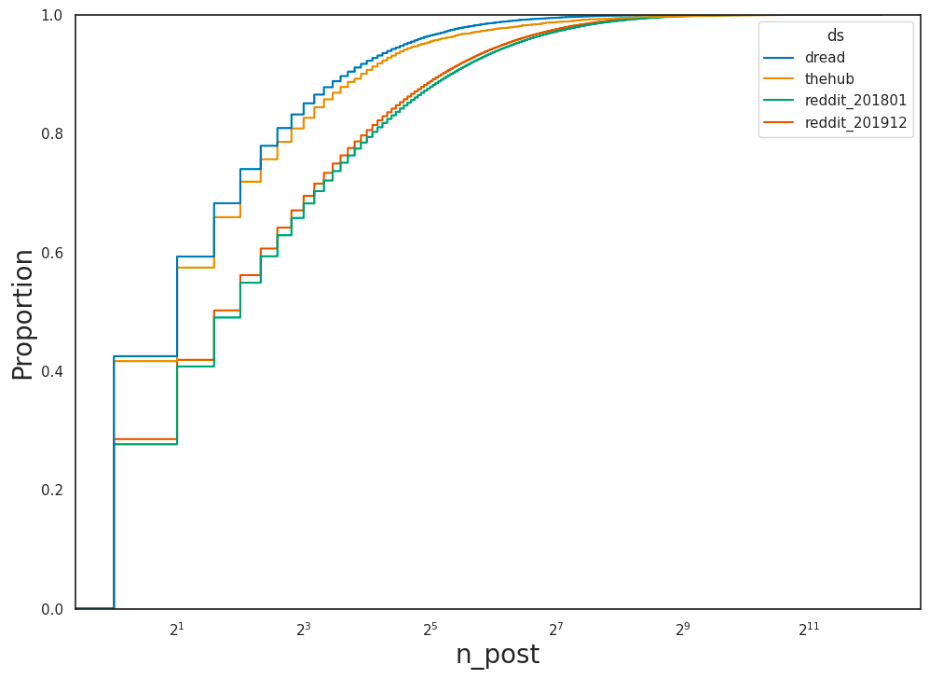
\includegraphics[width=\textwidth]{stylometryExtensions/figures/RedditPostCDF}
        \caption{Empirical Cumulative Distribution Function showing the proportion of authors having n\_post posts. Reddit has a much smaller proportion of authors with only one post.}
        \label{fig:stylometry_extensions:followingTrail:datasets:behaviors:posts}
    \end{subfigure}
    \begin{subfigure}{0.75\linewidth}
        \centering
        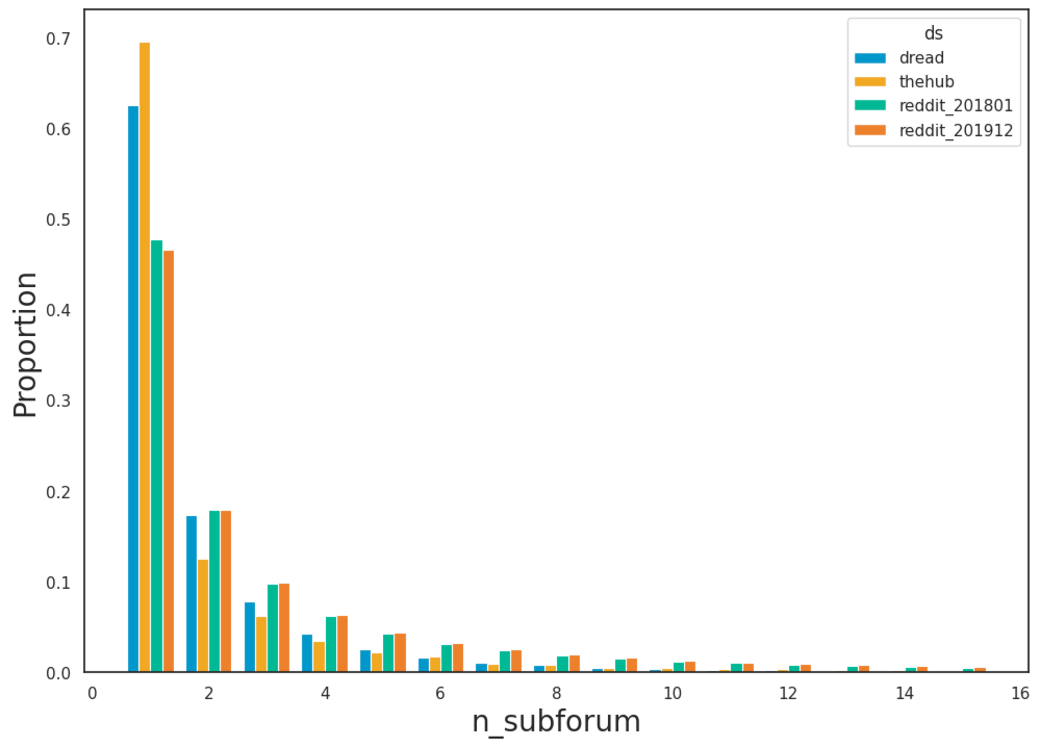
\includegraphics[width=\textwidth]{stylometryExtensions/figures/RedditSubforumCounts}
        \caption{Histogram of the number of subforums an author has posted in. Reddit has fewer authors posting on only one subforum.}
        \label{fig:stylometry_extensions:followingTrail:datasets:behaviors:subforums}
    \end{subfigure}
    \caption{User behaviors on Reddit, Dread, and TheHub.}
    \label{fig:stylometry_extensions:followingTrail:datasets:behaviors}
\end{figure}

As a first step to understanding the differences in the datasets, we aim to characterize the authors.
Figure~\ref{fig:stylometry_extensions:followingTrail:datasets:behaviors} provides two figures that capture distributions that characterize the user behaviors.
Figure~\ref{fig:stylometry_extensions:followingTrail:datasets:behaviors:posts} shows the cumulative distribution function of the number of posts per author.
We observe that Reddit has a much smaller proportion of authors with only one post.
This indicates that there are a larger proportion of authors posting on Darkweb forums with only a single post.
This may indicate that users create \textit{throwaway accounts}~\cite{leavitt2015throwaway} more frequently on the dark web as they desire greater anonymity.
Figure~\ref{fig:stylometry_extensions:followingTrail:datasets:behaviors:subforums} shows the histogram of the number of subforums a user has posted in.
This indicates that authors on Reddit may have interests in diverse topics, or the granularity of subforums is higher on Reddit.
Thus, even from a summary statistics perspective, there are fundamental differences in author behaviors across the clear and dark web forums.
However, it is unclear how these differences at the macro level will affect the generalization capabilities of LUAR.

\subsubsection{Preprocessing for Author Identification}
